\chapter{Évolution Différentielle}

\section{Introduction}

L'Évolution Différentielle (ED) est un algorithme évolutionnaire développé par Storn et Price \cite{Storn1995} en 1995. Il est versatile et relativement simple à implémenter et utiliser, ce qui en fait un outil essentiel dans toute boite à outils d'optimisation. Comme toutes les techniques évolutionnaires, le principe de l'évolution différentielle repose sur la génération d'une population de $N_P$ solutions (ou "vecteurs") qui permettent d'évaluer une fonction objectif à des points initiaux distribués aléatoirement dans un espace de recherche borné selon l'utilisateur. Ces points sont "perturbés" dans les générations successives de la population pour essayer de trouver des solutions extrémisant la fonction objectif. L'une des caractéristiques qui font la particularité de tout algorithme évolutionnaire est l'opération utilisée pour effectuer cette perturbation. Dans le cas de l'évolution différentielle, on perturbe une solution avec la différence de deux autres vecteurs de la population, multipliée par un facteur F, c'est l'opération dite de "mutation" comme est présenté dans la figure \ref{fig:deflowchart}. Ce nouveau vecteur subit une opération de croisement avec le vecteur initial pour produire le vecteur d'essai qui est comparé avec le vecteur de même indice dans la population. Ceci est refait jusqu'à ce que tous les vecteurs de la population soient comparés avec un vecteur d'essai (soit $N_P$ fois), créant la génération suivante. L'algorithme continue de créer de plus en plus de générations jusqu'à ce qu'un critère d'arrêt est satisfait. Souvent c'est un nombre de générations maximal ou une valeur de tolérance pour la variation de la fonction objectif.

\begin{figure}[H]
  \begin{center}
    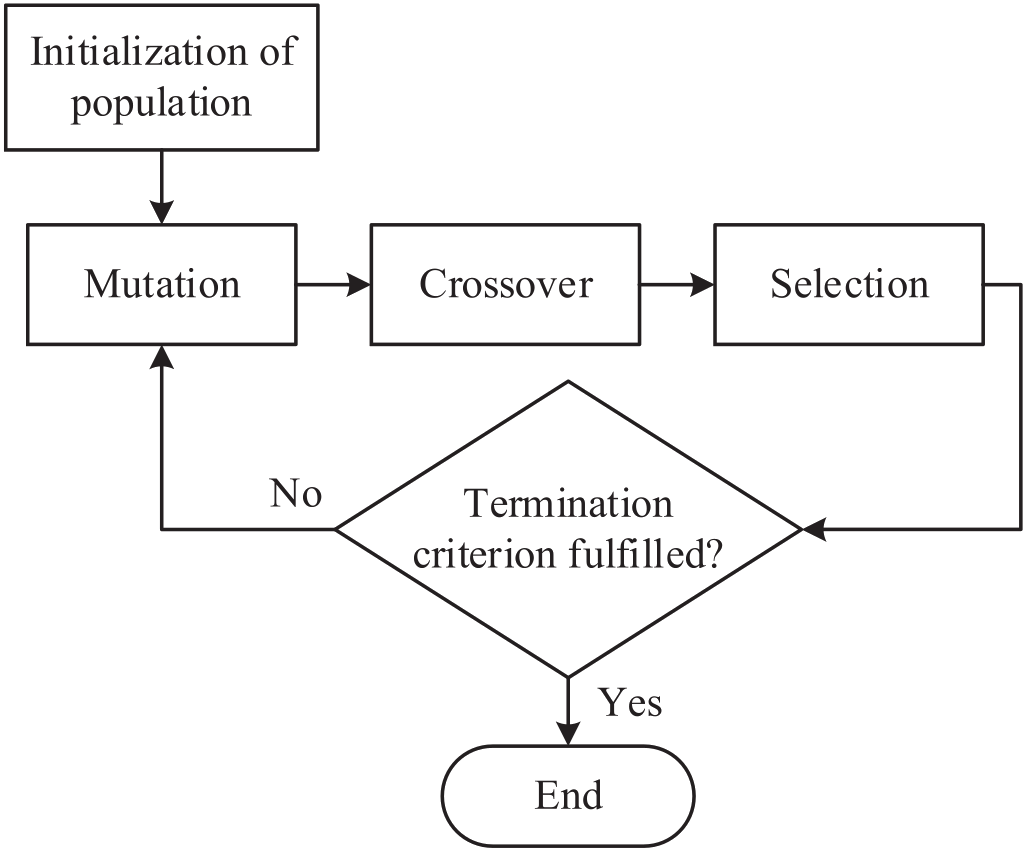
\includegraphics[width=.6\textwidth]{resources/DE.png}
    \caption{Organigramme des étapes de l'Évolution Différentielle \cite{Chin2019}}
    \label{fig:deflowchart}
  \end{center}
\end{figure}

\section{Description de l'algorithme}

\subsection{Initialisation}

\begin{wrapfigure}{r}{0.5\textwidth}
  \vspace*{-10pt} 
  \begin{center}
    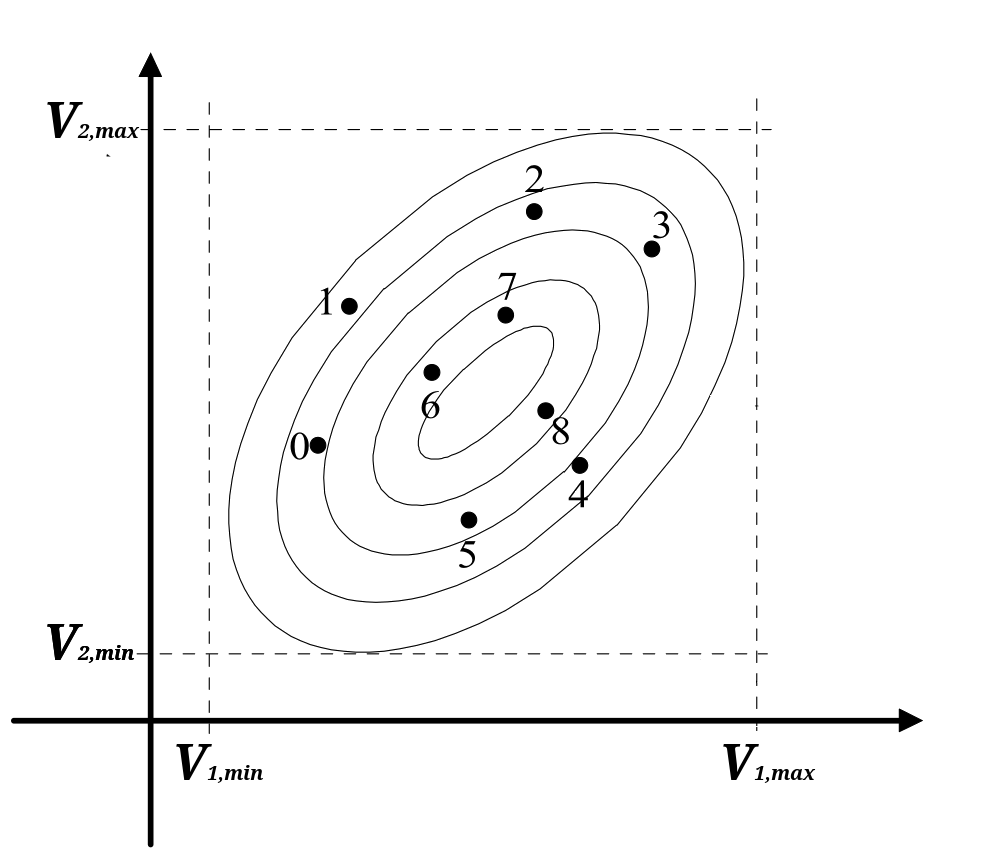
\includegraphics[width=\textwidth]{resources/initpop.png}
    \caption{Exemple d'une population initialisée dans un espace de recherche à deux dimensions. Dans ce cas $D = 2$, $N_P = 9$ et l'indice de génération $g = 0$ puisqu'il s'agit de la population initiale}
    \label{fig:initpop}
  \end{center}
\end{wrapfigure}

La convergence des techniques d'optimisation non-linéaires est toujours conditionnée par un "bon" choix des conditions initiales. Dans le cas de l'évolution différentielle, il s'agit de l'ensemble des vecteurs constituants la population initiale. Si un vecteur solution quelconque se constitue de $D$ paramètres, notre espace de recherche est dit à $D$ dimensions, ce qui fait que notre population initiale se compose de $N_P$ vecteurs à $D$ éléments. Mais pour pouvoir effectuer l'initialisation de la population, les bornes de l'espace de recherche doivent être spécifiées. Chacun des $D$ paramètres doit avoir une borne supérieure et inférieure, ce qui fait un total de $2 \times D$ valeurs pour spécifier complètement les limites de l'espace. Reste le mécanisme utilisé pour effectivement générer les vecteurs dans cet espace borné. Pour couvrir entièrement et uniformément cet espace, il faut, pour chaque paramètre de chaque vecteur, générer aléatoirement et uniformément une valeur comprise dans la fourchette déterminée par un générateur de nombres aléatoires. En considérant que l'indice $j$ associé à un vecteur $V$ désigne le $j-$ème paramètre, on peut accomplir ceci avec la formule \ref{eq:popinit}. 

\begin{equation}
  \label{eq:popinit}
  V_j = V_{\text{min},j} + \text{rand}[0, 1](V_{\text{max},j} - V_{\text{min},j})
\end{equation} 

On suppose avoir accès à une fonction $\text{rand}[0, 1]$, qui joue le rôle du générateur de nombres aléatoire uniformes et que $0 \leq \text{rand}[0, 1] < 1$. 
$V_{\text{min},j}$ et $V_{\text{max},j}$ sont les bornes inférieures   et supérieures du $j-$ème paramètres, respectivement. Figure \ref{fig:initpop} montre un exemple d'une population initialisée dans un espace de recherche 2 dimensionnel. Les contours sont les \textit{"isolignes"} de la fonction objectif, le minimum global doit être à l'intérieur de la fourchette spécifiée. 
\clearpage

\subsection{Mutation}

\begin{wrapfigure}{r}{.5\textwidth}
%  \vspace*{-50pt}
  \begin{center}
    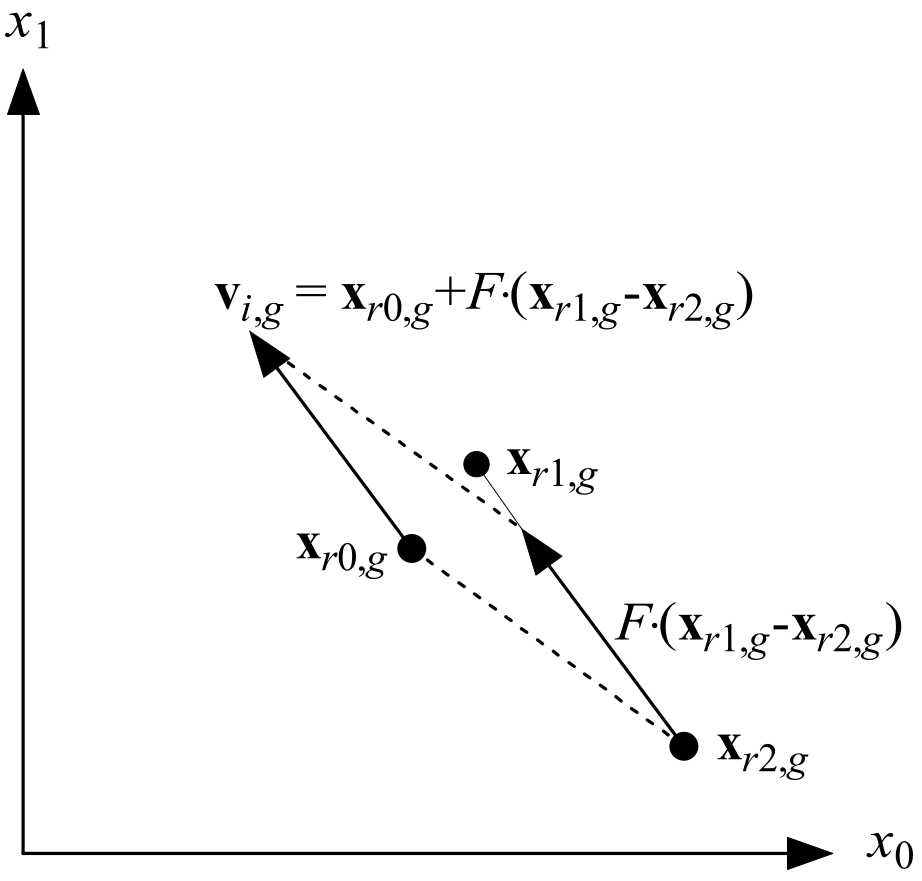
\includegraphics[width=.9\textwidth]{resources/mutant.png}
    \caption{L'operation de mutation differentielle ajoute $F (V_{r1,gen} - V_{r2,gen})$ au vecteur de base $V_{base,gen}$ pour produire un mutant $M_{i,gen}$}
  \end{center}
  \label{fig:mutant}
%  \vspace*{-30pt}
\end{wrapfigure}

Après l'initialisation de la population, l'ED modifie, croise et recombine la population pour produire des vecteurs d'essai (un nombre $N_P$ de ces vecteurs) qui seront comparés avec les vecteurs cibles qui leurs correspondent dans la population. La \textit{Mutation} dans l'ED est en fait une "mutation différentielle". Elle consiste a ajouter la différence de deux vecteurs choisis aléatoirement de la population, multipliée par un facteur de pondération ou "Facteur de Mutation", à un troisième vecteur de base distinct. Cette opération produit un vecteur mutant $M$ selon l'équation \ref{eq:mutant}. L'indice $i$ indique le $i$-ème vecteur de la population, et $gen$ la génération où l'on est. 
Il n'y a pas de limite dure sur le Facteur de Mutation $F$, mais les valeurs supérieures à $1$ sont rarement considérées. Dans notre cas, on considère que $F \in [0, 1]$. Il existe plusieurs stratégies pour choisir le $V_{base}$, le seul prérequis étant qu'il soit distinct du vecteur cible. Dans ce travail nous utiliserons exclusivement le choix du vecteur ayant la meilleure qualité ou valeur de "fitness" calculée par la fonction objectif. Les vecteurs de la différence $V_{r1,gen}$ et $V_{r2,gen}$ sont choisis aléatoirement de la population pour chaque vecteur mutant et ne doivent qu'être distincts l'un de l'autre et des vecteurs cible $V_{i, gen}$ et de base $V_{base, gen}$.

\begin{equation}
  \label{eq:mutant}
  M_{i,gen} = V_{base,gen} + F (V_{r1,gen} - V_{r2,gen})  
\end{equation}

\subsection{Croisement}
La opération de mutation est suivie d'un croisement ou \textit{recombinaison discrète}. Elle consiste à construire le vecteur d'essai $T_{i,gen}$ à partir des éléments (i.e. paramètres) de deux vecteurs différents selon une probabilité spécifiée. Chaque élément $j$ du vecteur d'essai est choisi selon la formule \ref{eq:cross}
\begin{equation}
  \label{eq:cross}
  T_{j,i,gen} =
  \begin{cases}
    M_{j,i,gen} & \text{si}\ \text{rand}[0, 1] \leq CR\ \text{ou}\ j = j_{rand}\\
    V_{j,i,gen} & \text{sinon}
  \end{cases}
\end{equation}
$CR \in [0,1]$ détermine la probabilité que le paramètre provienne du vecteur mutant tant que $\text{rand}[0, 1]$ est effectivement un générateur aléatoire uniforme. Le taux de croisement $CR$ est l'un des paramètres spécifiés par l'utilisateur au début. Un nombre aléatoire $j_{rand}$ est aussi choisi tel que $0 \leq j_{rand} < D$ pour s'assurer que le nouveau vecteur d'essai ne duplique pas complètement le vecteur cible $V_{i,gen}$.

\subsection{Pénalité}

\subsection{Sélection}
Si le vecteur d'essai $T_{i,gen}$ est évalué à une valeur inférieure par la fonction objectif $f$ au vecteur cible $V_{i,gen}$, il le remplace dans la génération suivante (i.e. $gen + 1$). Sinon le vecteur cible survit à la sélection et retient sa place dans la génération suivante (équation \ref{eq:selection}).
Quand la nouvelle population est complète, le processus de mutation, croisement et sélection est renouvelé jusqu'à ce qu'un critère d'arrêt est vérifié (e.g. un nombre maximal de générations $gen_{max}$)

\begin{equation}
  \label{eq:selection}
  V_{i, gen + 1} =
  \begin{cases}
    T_{i,gen} & \text{si}\ f(T_{i,gen}) \leq f(V_{i,gen})\\
    V_{i,gen} & \text{sinon}
  \end{cases}
\end{equation}

%\section{Application aux modèles simple et double diodes}

%\section{Métaheuristique}

 
